\documentclass[a4paper, 12pt]{article}
\usepackage[polish]{babel}
\usepackage[utf8]{inputenc}
\usepackage[T1]{fontenc}
\usepackage{graphicx}
\usepackage{float}
\usepackage{hyperref}
\usepackage{multirow}
\usepackage{array}
\usepackage{bookmark}
\usepackage{geometry}
\geometry{a4paper, margin=2cm}

\title{Protokół z ćwiczeń cz. II: Oszacowanie obciążenia genetycznego}
\author{Mikołaj Mieszko Charchuta}
\date{14.02.2025}

\begin{document}

\maketitle

\section{Wprowadzenie}
Celem badania było zastosowanie metod ze świeżej publikacji \cite{Speak2024} do oszacowania obciążenia genetycznego u dwóch blisko spokrewnionych gatunków ptaków: biegusa łyżkodziobego (\textit{Calidris pygmaea}) oraz biegusa rdzawoszyjego (\textit{Calidris ruficollis}). Biegus łyżkodzioby jest gatunkiem krytycznie zagrożonym wyginięciem, co czyni go idealnym obiektem do badania wpływu małej liczebności populacji na erozję genetyczną. Podchodząc do analiz, spodziewam się, że analizowany osobnik (\textit{C. pygmaea}) będzie miał wyższe obciążenie genetyczne niż osobnik \textit{C. ruficollis}.

\section{Materiały i Metody}
Schematyczny przebieg podsekcji 2.1-3 przedstawiono na Rysunku \ref{fig:workflow1}. Do analizy wykorzystano dane sekwencjonowania genomowego po osobniku z obu gatunków: biegusa łyżkodziobego (C\_pyg\_26) oraz biegusa rdzawoszyjego (C\_ruf\_09). Dane ograniczono do analizy scaffoldu 1 genomu referencyjnego biegusa łyżkodziobego. 

\begin{figure}[H]
    \centering
    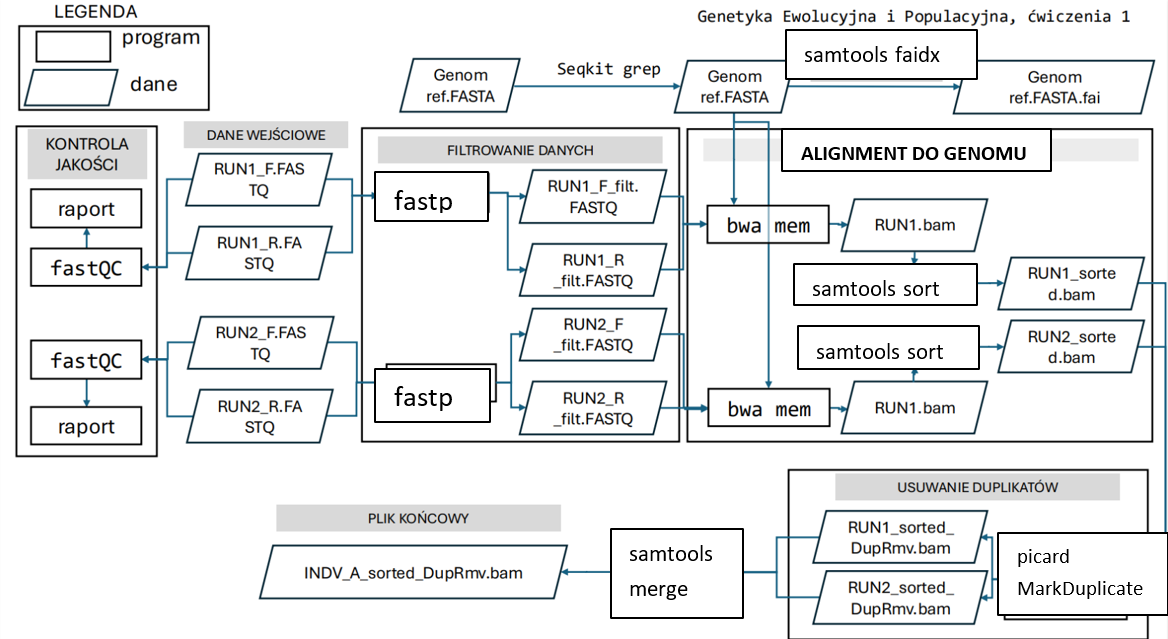
\includegraphics[width=\textwidth]{img/workflow1.png}
    \caption{Workflow 1: Przygotowanie danych}
    \label{fig:workflow1}
\end{figure}

\subsection{Przygotowanie danych}
Sekwencje scaffoldu 1 wyodrębniono z genomu referencyjnego za pomocą narzędzia \textbf{seqkit grep}. Plik FASTA scaffoldu 1 zindeksowano przy użyciu \textbf{samtools faidx}. 
Dane sekwencjonowania odczytów zostały pobrane z NCBI SRA (próbki SRS3209979 i SRS3209990, oraz odpowiednio przebiegi: SRR7054135\&SRR7054162 i SRR7054133\&SRR7054147). 
\subsection{Analiza jakości odczytów}
Jakość odczytów przed i po filtrowaniu była wysoka, choć wykryto regiony o niskiej jakości, prawdopodobnie związane z błędami sekwencjonowania. Odczyty sprawdzono oraz przefiltrowano za pomocą narzędzia \textbf{fastQC}. Wyniki kontroli i filtrowania przedstawiono w Tabeli \ref{tab:quality_analysis}. 
\subsection{Mapowanie odczytów}
 Mapowanie odczytów do scaffoldu 1 wykonano za pomocą Burrows-Wheeler Aligner - \textbf{bwa mem}. Pliki pośrednie usunięto, a pliki BAM posortowano programem \textbf{samtools sort}. Duplikaty usunięto za pomocą \textbf{picard MarkDuplicates}. Końcowy plik .bam uzyskano z obu powtórzeń sekwencjonownia za pomocą \textbf{samtools merge}.

\begin{table}[H]
    \centering
    \begin{tabular}{|c|c|p{5cm}|p{5cm}|}
        \hline
        Osobnik & Filtrowanie & Run 1 & Run 2 \\
        \hline
        \multirow{2}{*}{C\_ruf\_09} & Przed & 
        Długość odczytów - 125 pz. Wyniki w większości bardzo dobre. Jedna sekwencja jest nadreprezentowana. Blastowana daje różne dziwne wyniki… ale najpewniej to primer Illuminy. Na płytce znajduje się miejsce z sekwencjami o niskiej jakości. & 
        Stała długość odczytów - 125 pz. Wyniki w większości bardzo dobre. Jedna sekwencja jest nadreprezentowana. To samo. \\
        \cline{2-4}
        & Po & 
        Odczyty po filtracji mają długość od 42 do 125 pz, głównie > 123 pz. Filtrowanie usunęło tylko małą część nadreprezentowanych sekwencji. & 
        Odczyty po filtracji mają długość od 42 do 125 pz, głównie > 123 pz. Filtrowanie usunęło tylko małą część nadreprezentowanych sekwencji. \\
        \hline
        \multirow{2}{*}{C\_pyg\_26} & Przed & 
        Generalnie dobre wyniki. Doszło jednak do problemu na płytce. Te nadreprezentowane sekwencje są spodziewane? Więcej odczytów zawiera GC na poziomie 42\% niż przewidziano w teoretycznym rozkładzie. & 
        Wyniki dobre, wykryto nadmiar nadreprezentowanych sekwencji. Więcej odczytów zawiera GC na poziomie 42\% niż przewidziano w teoretycznym rozkładzie. \\
        \cline{2-4}
        & Po & 
        Usunięto nadreprezentatywne sekwencje. Liczba odczytów z 42\% zawartością GC nadal wysoka. & 
        Nadal dużo odczytów z 42\% zawartością GC. Usunięto nadreprezentowane sekwencje. \\
        \hline
    \end{tabular}
    \caption{Analiza jakości odczytów sekwencjonowania}
    \label{tab:quality_analysis}
\end{table}

\begin{figure}[H]
    \centering
    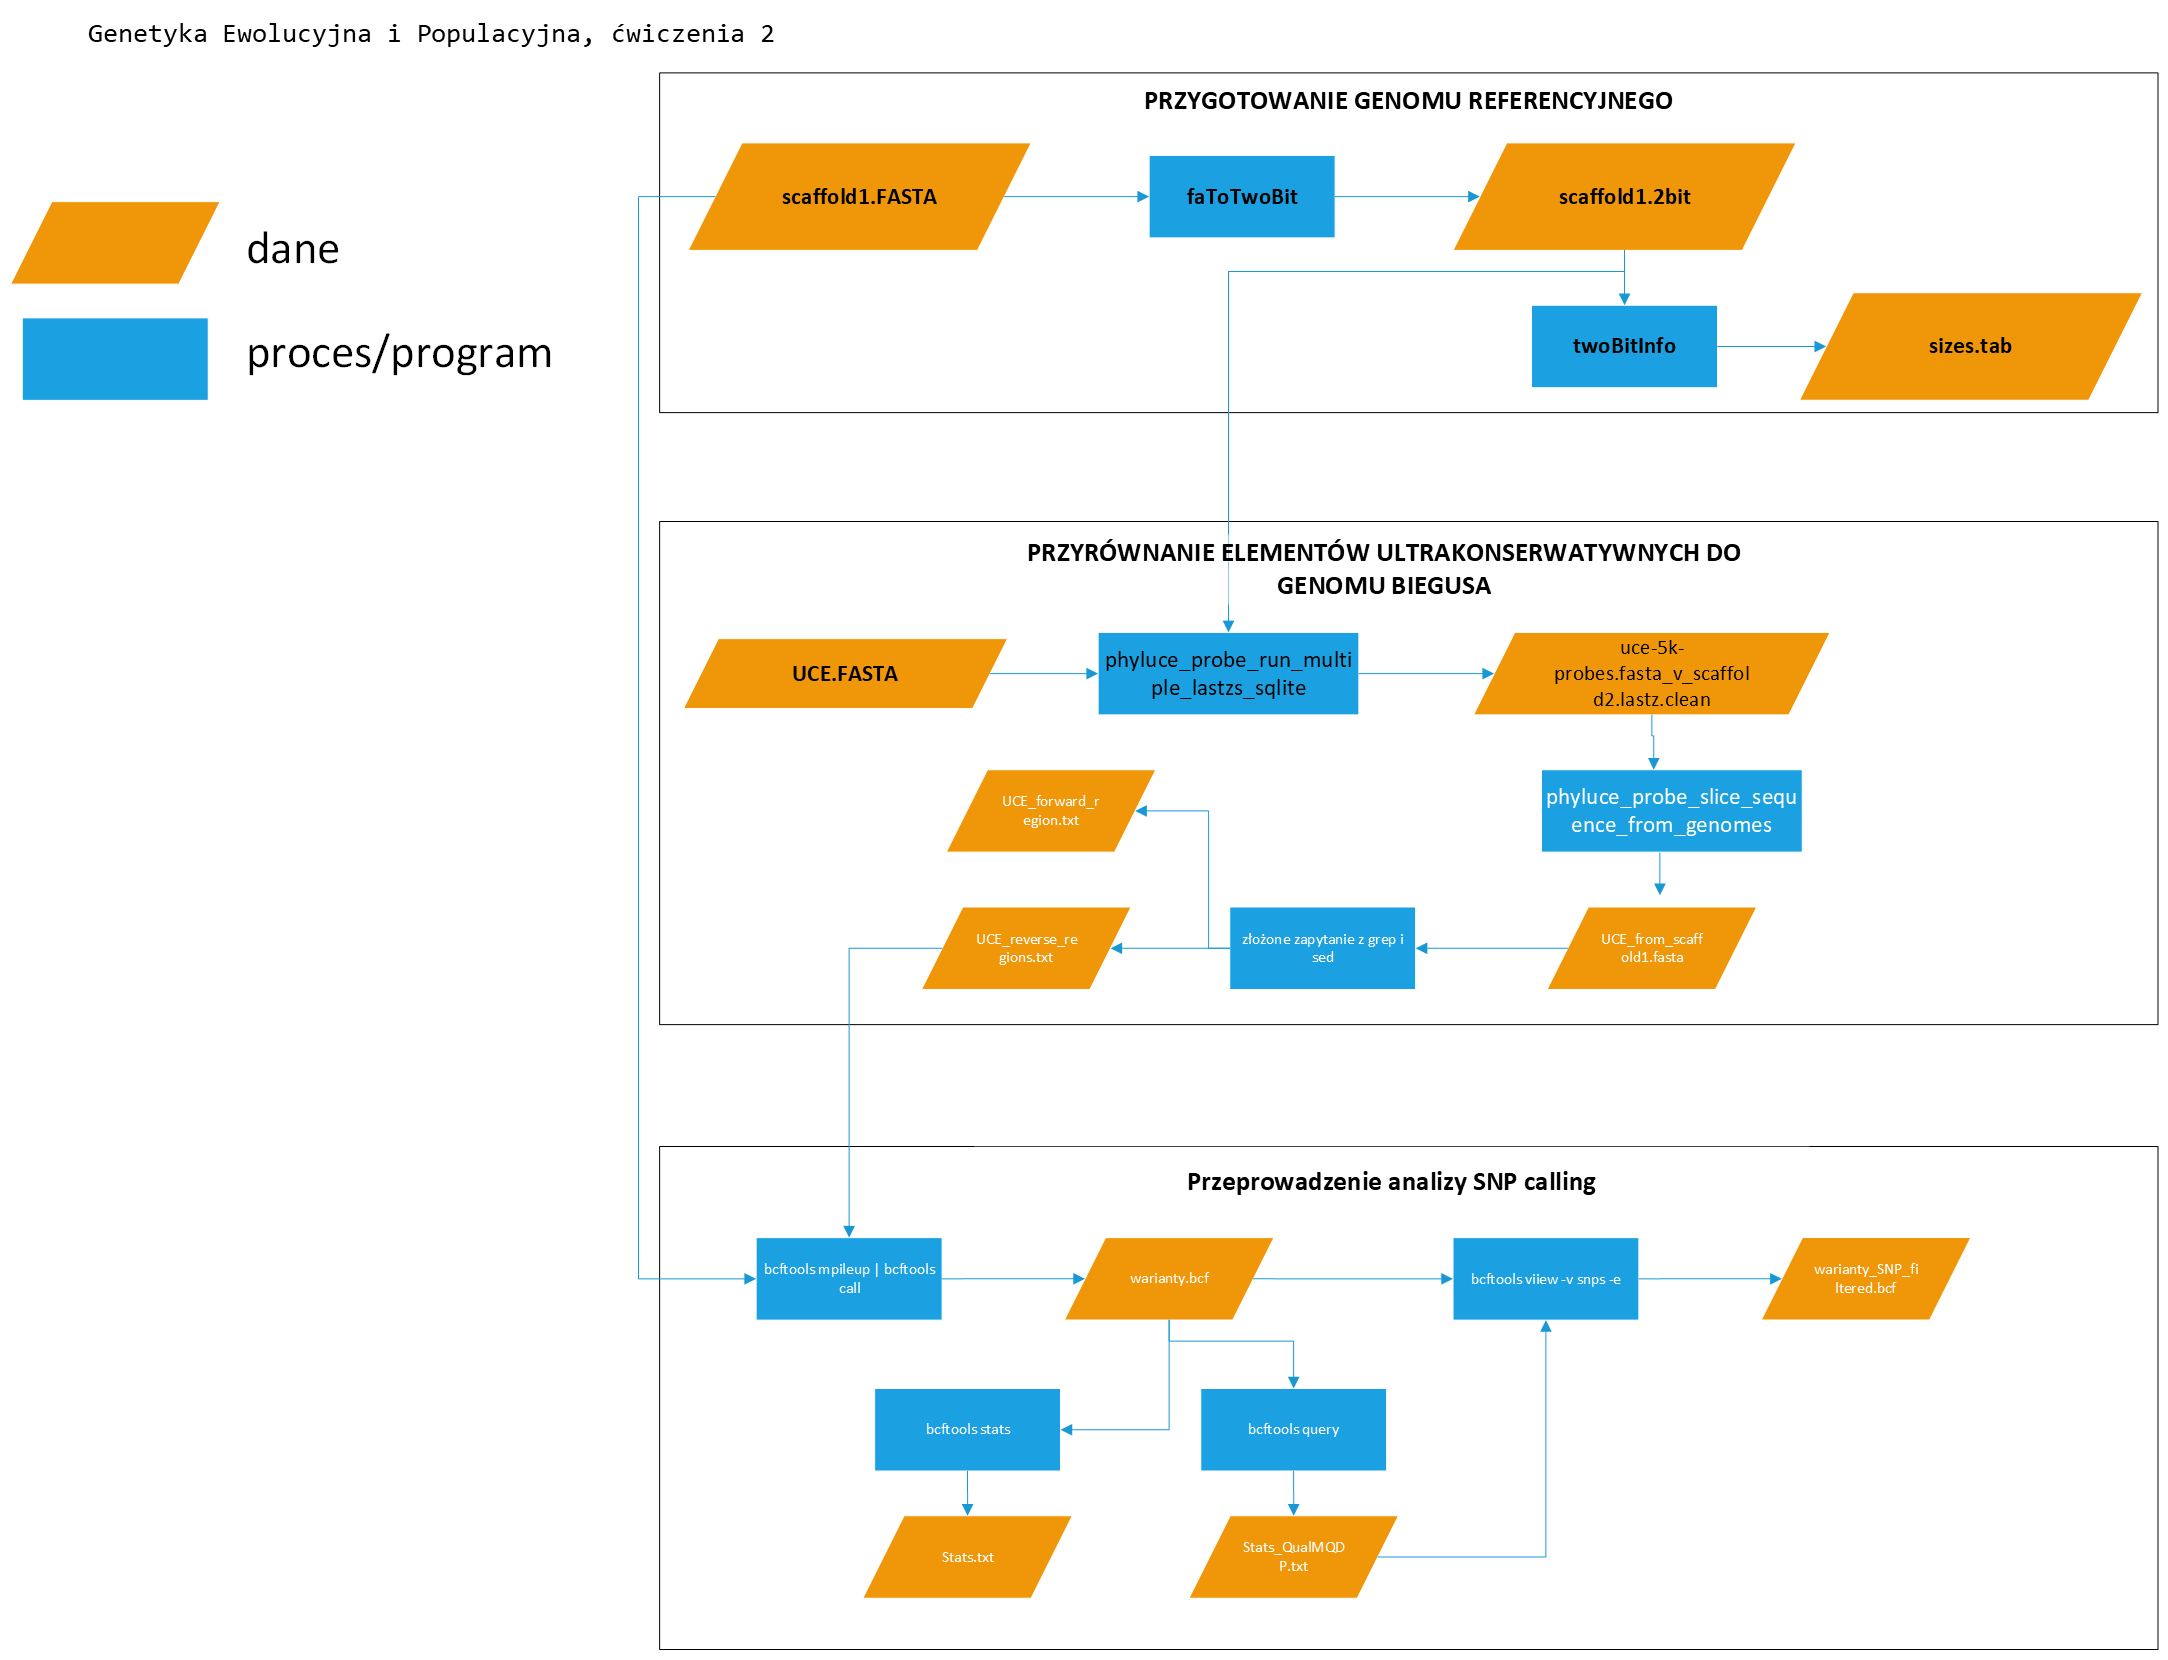
\includegraphics[width=\textwidth]{img/workflow2.png}
    \caption{Workflow 2: Identyfikacja SNP}
    \label{fig:workflow2}
\end{figure}
\subsection{SNPy}
Workflow 2 przedstawia proces identyfikacji SNP (Single Nucleotide Polymorphisms).
\subsubsection{Konwersja do formatu .2bit}
Konieczna dla optymalizacji pamięci. Wykorzystano narzędzie \textbf{faToTwoBit}.
\subsubsection{UCE}
Po przekonwertowaniu danych do formatu .2bit do danych od biegusów przyrównano elementy ultrakonserwatywne programem \textbf{LASTZ} w frameworku pakietu \textbf{phyluce} wyodrębniając UCE z analizowanych scaffoldów wraz z 1kbp sąsiadujących z UCE. Wszystkie wyodrębnione sekwencje miały orientację REVERSE.
\subsubsection{SNP calling}
 Narzędzie \textbf{bcftools mpileup} generuje plik w formacie pileup, który zawiera informacje o odczytach zmapowanych do genomu referencyjnego. Plik pileup zawiera szczegóły na temat pozycji w genomie, alleli referencyjnych i alternatywnych, jakości odczytów oraz liczby odczytów wspierających każdy allel. Narzędzie \textbf{bcftools call}.analizuje te informacje o odczytach i decyduje, czy dana pozycja jest polimorficzna (czyli czy występuje wariant).

\subsubsection{Filtracja SNPów}
Warianty zostały następnie przefiltrowane przy użyciu \textbf{bcftools} i informacji uzyskanych z wykresów \ref{fig:qualmqdp_pyg} i \ref{fig:qualmqdp_ruf}, w celu usunięcia niskiej jakości SNP oraz SNP o niskiej częstości alleli. Ostateczne zestawy SNP zostały zapisane w formacie VCF i wykorzystane do dalszych analiz.

\begin{figure}[H]
    \centering
    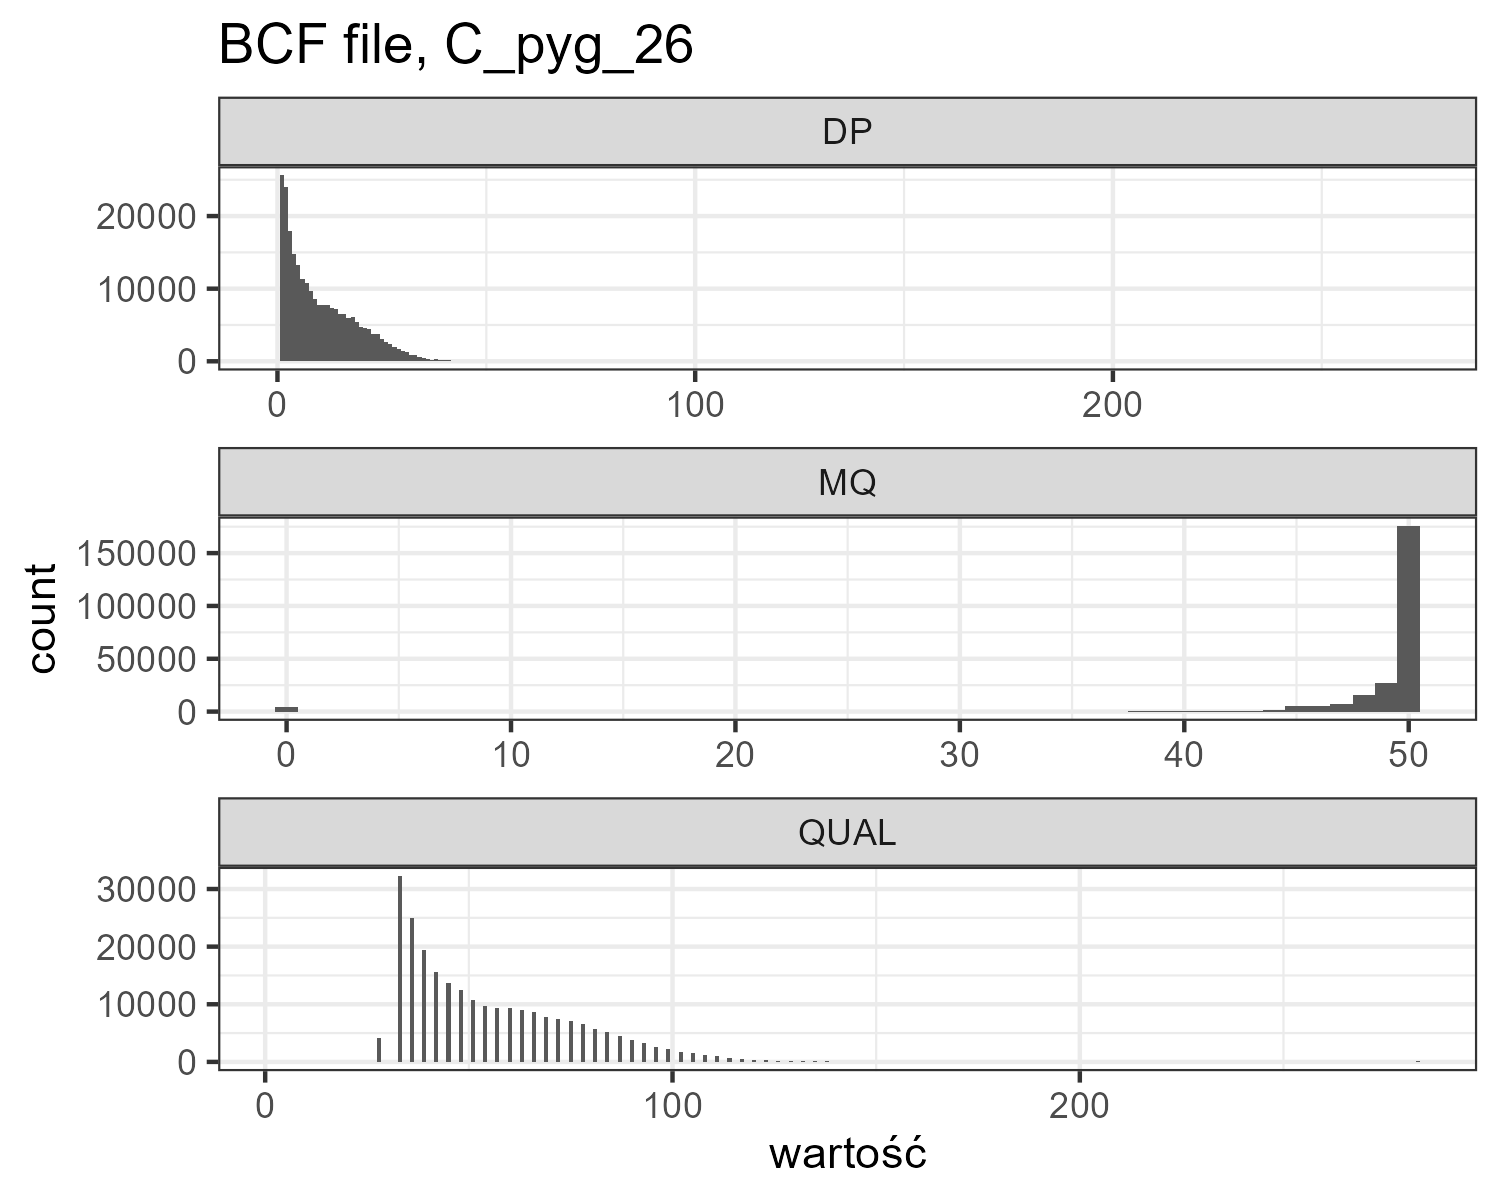
\includegraphics[width=0.49\textwidth]{img/Stats_QualMQDP_C_pyg_26.png}
    \caption{Statystyki jakości, MQ i DP dla biegusa łyżkodziobego.}
    \label{fig:qualmqdp_pyg}
\end{figure}
\hfill
\begin{figure}[H]
    \centering
    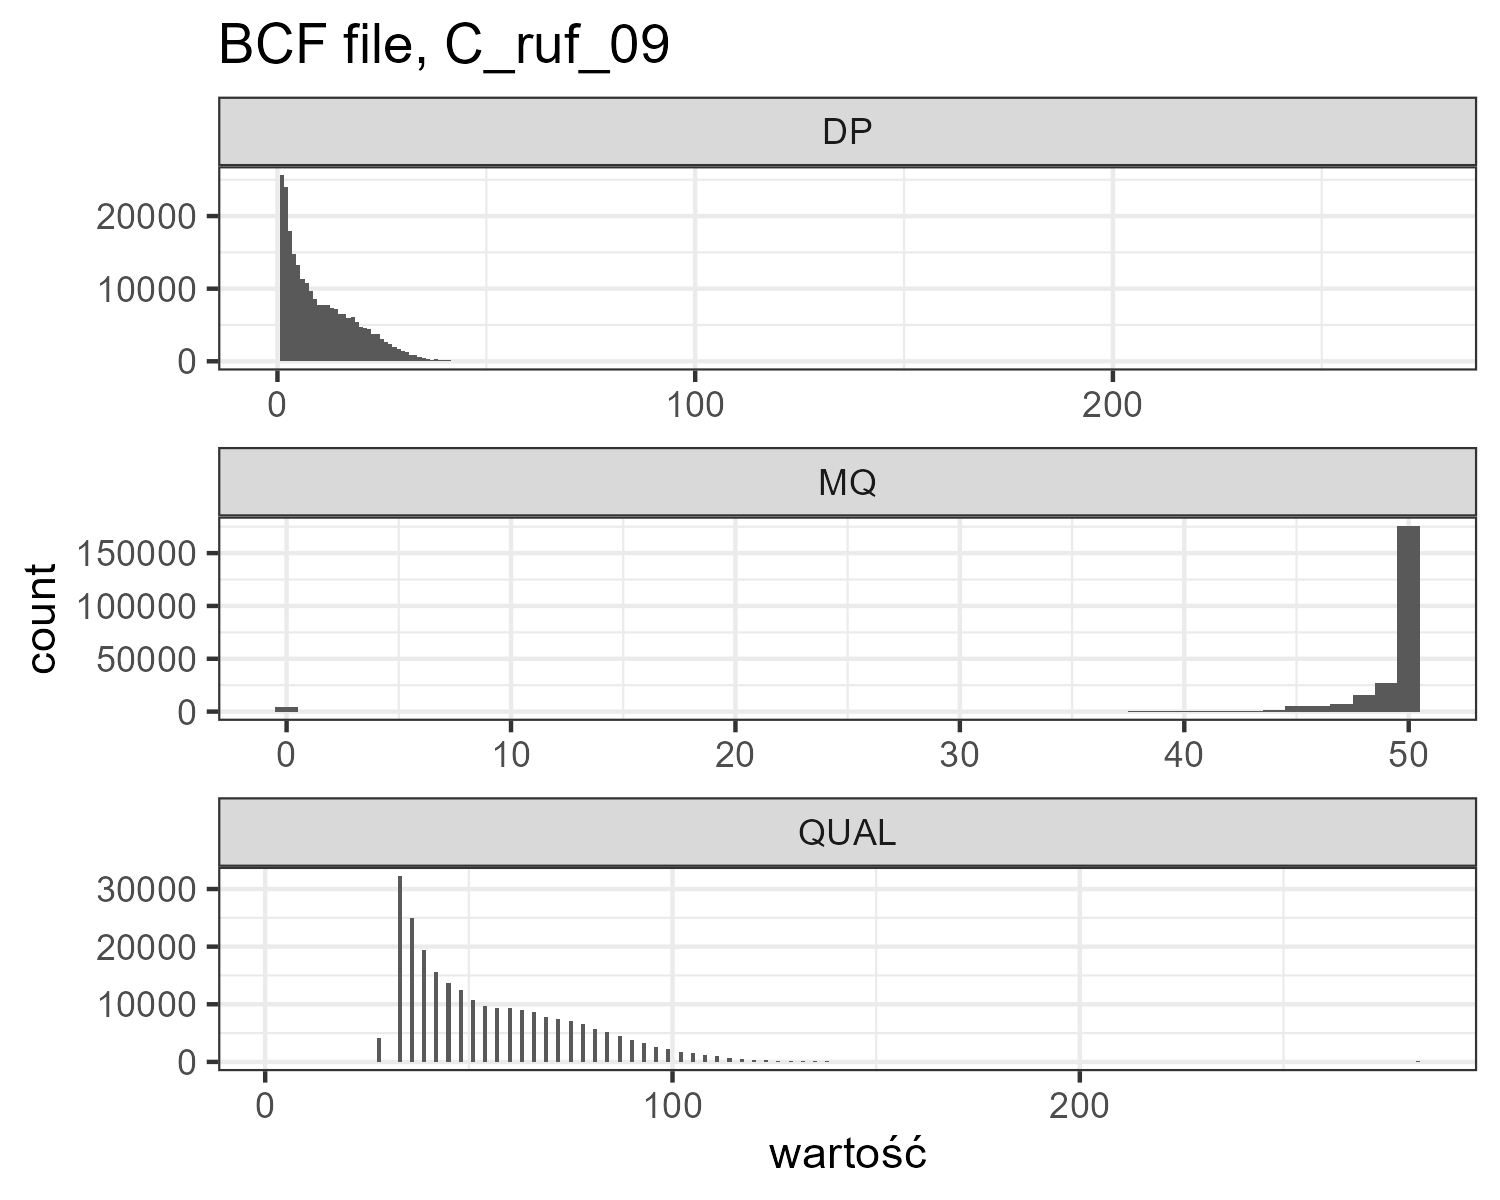
\includegraphics[width=0.49\textwidth]{img/Stats_QualMQDP_C_ruf_09.png}
    \caption{Statystyki jakości, MQ i DP dla biegusa rdzawoszyjego.}
    \label{fig:qualmqdp_ruf}
\end{figure}



\begin{figure}[H]
    \centering
    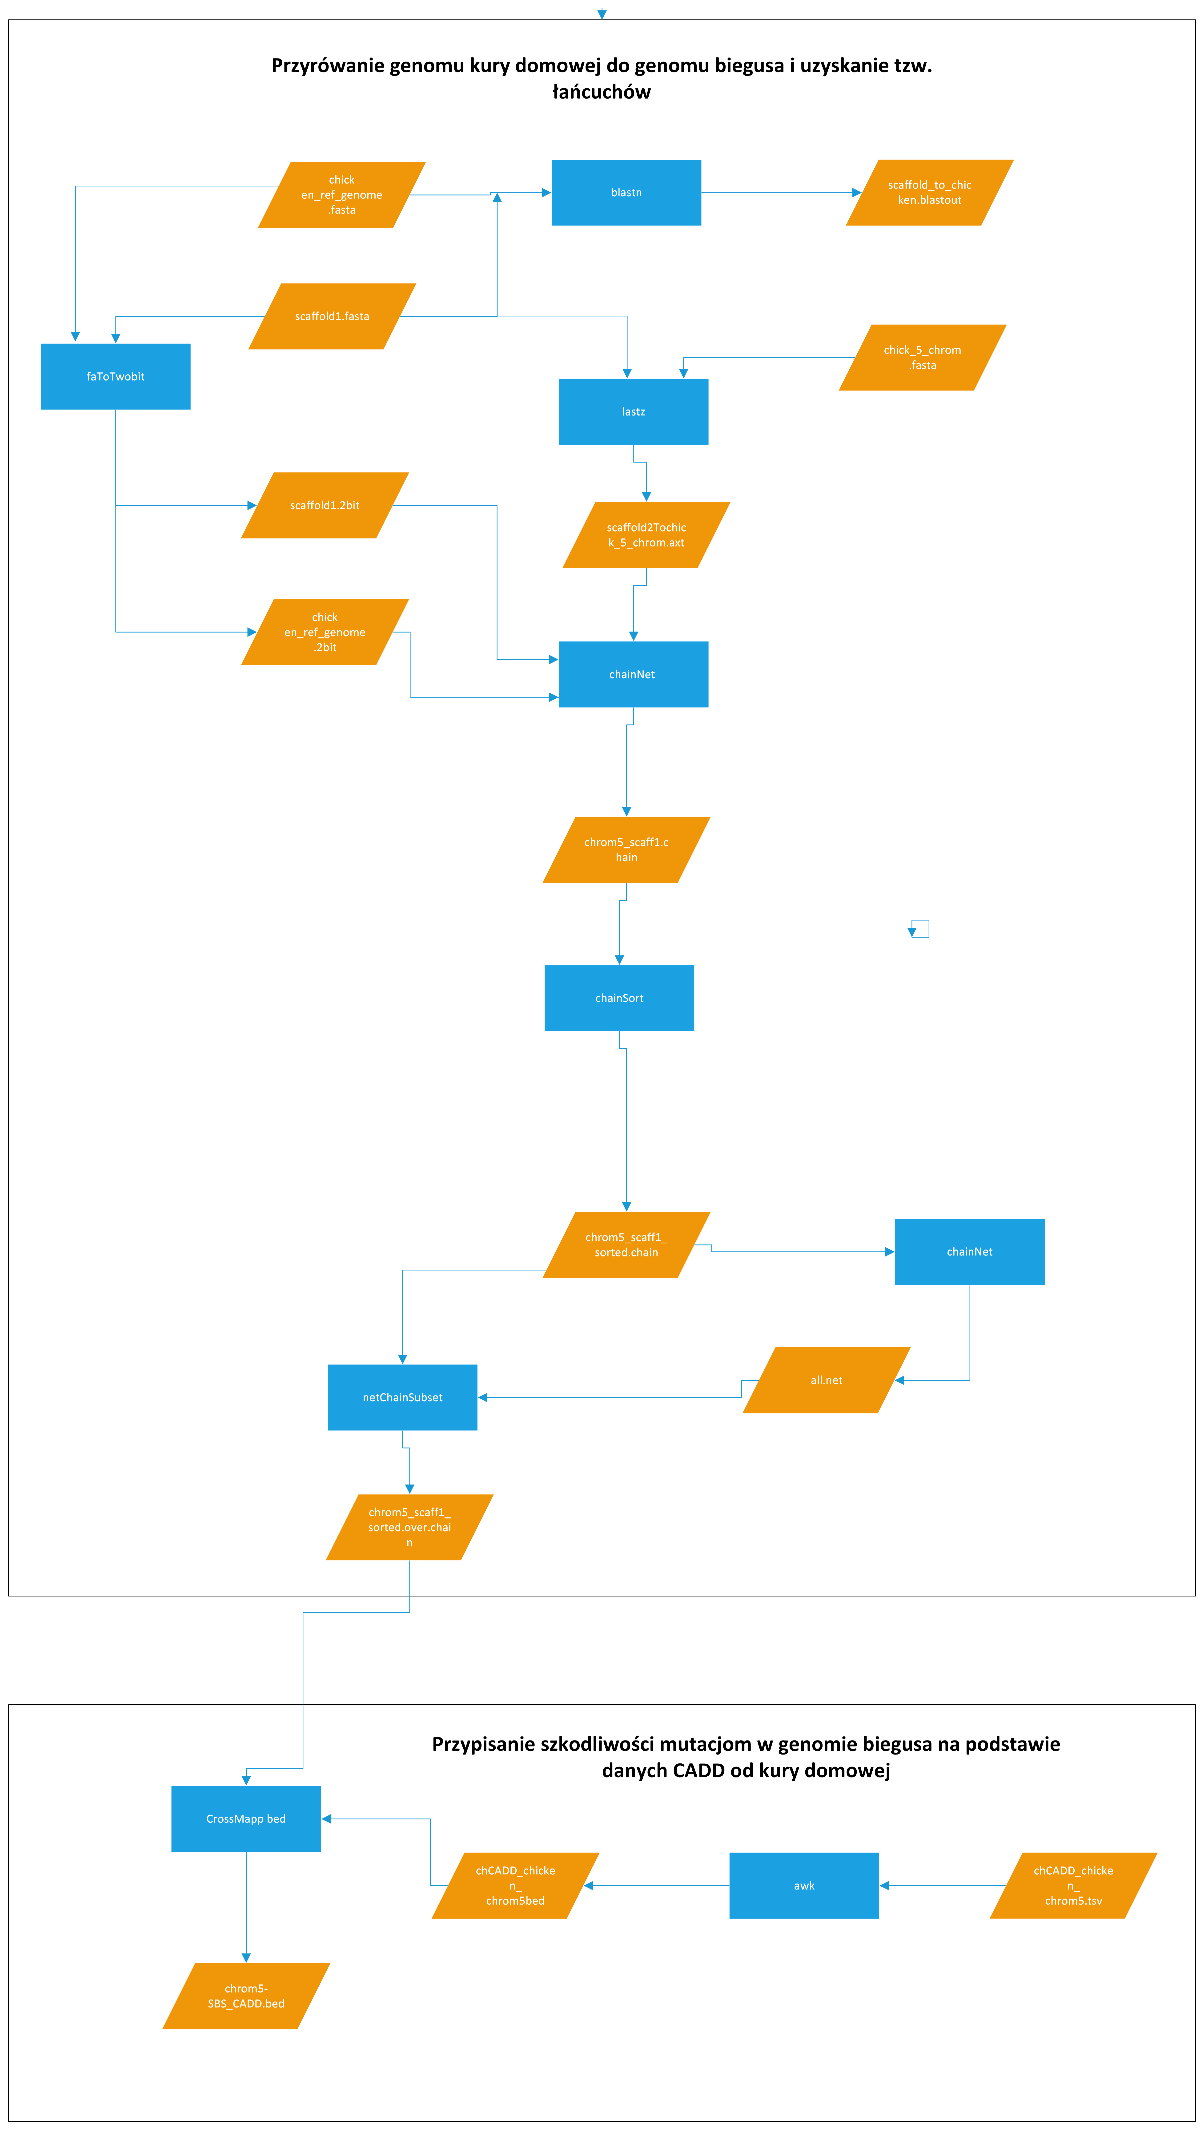
\includegraphics[width=0.8\textwidth]{img/workflow4.png}
    \caption{Workflow 4: }
    \label{fig:workflow4}
\end{figure}

\subsection{Chaining}
Wynik działania programu \textbf{LASTZ} potraktowano komendą \textbf{axtChain} by złączyć je w większe i bardziej spójne bloki (tzw. 
łańcuchy, chains). Różnica przed i po chainingu przedstawiona jest na Rysunku \ref{fig:before_chaining} i \ref{fig:after_chaining}.

\begin{figure}[H]
    \centering
    \begin{minipage}{0.49\textwidth}
        \centering
        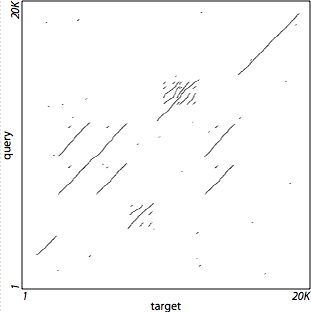
\includegraphics[width=\textwidth]{img/before_chaining.png}
        \caption{Wynik działania programu LASTZ przed chainingiem.}
        \label{fig:before_chaining}
    \end{minipage}
    \hfill
    \begin{minipage}{0.49\textwidth}
        \centering
        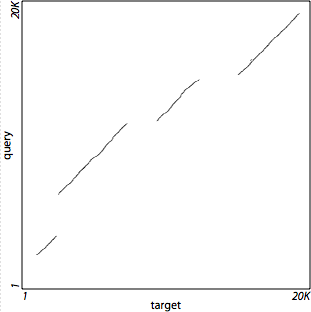
\includegraphics[width=\textwidth]{img/after_chaining.png}
        \caption{Wynik działania programu LASTZ po chainingu.}
        \label{fig:after_chaining}
    \end{minipage}
\end{figure}
Utworzone łańcuchy powinny być pofiltrowane. W nowej wersji protokołu w wyniku filtrowania z 1666 łańcuchów pozostało... 256. Wynik filtrowania przedstawiono na Rysunku \ref{fig:filtered_chains}. Zdziwiło mnie to, bo wcześniej filtrowanie usuwało tylko 5 łańcuchów, a teraz usunięto 1410, ale widzę, że dwóm innym studentom pracującym na scaffoldzie 1 również usunęło dużo łańcuchów, więc może to być wynik poprawnego działania programu.

\begin{figure}[H]
    \centering
    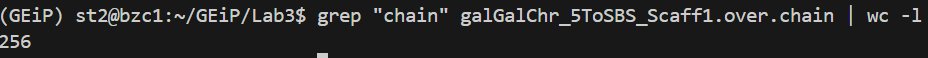
\includegraphics[width=0.8\textwidth]{img/maybe_erronously_filtered.png}
    \caption{Wynik filtrowania łańcuchów.}
    \label{fig:filtered_chains}
\end{figure}

\subsection{Przypisanie szkodliwości wariantom}
Do przypisania szkodliwości wariantom wykorzystano narzędzie \textbf{CADD}, a konkretnie jego model opracowany dla kury (\textit{Gallus gallus}) z publikacji \cite{Gro2020}. CADD (ang. Combined Annotation Dependent Depletion) to narzędzie oparte na porównaniu właściwości substytucji (mutacji utrwalonych w linii prowadzącej do człowieka) z właściwościami wymsymulowanych mutacji. Zakłada, że szkodliwe mutacje nie będą pojawiać się wśród substytucji, natomiast będą w danych symulowanych. Właściwości, które porównywane są pomiędzy tymi zbiorami danych, to m.in. informacje o zakonserwowaniu sekwencji (z przyrównania genomów wielu gatunków), poziom ekspresji genów, odległość od granicy egzonu, dane eksperymentalne, informacje o asocjacjach etc. Porównuje się symulowane mutacje z takimi, które obecne są w naturalnych populacjach i w ten sposób trenuje się model. Oszacowane wartości korelują z szacowaną eksperymentalnie patogenicznością mutacji i mogą być obliczone zarówno dla fragmentów kodujących, jak i niekodujących. Wyniki analizy przedstawiono na Rysunkach \ref{fig:cadd_pyg} i \ref{fig:cadd_ruf}.

\section{Wyniki}
\subsection{Analiza jakości odczytów}
Jakość odczytów przed i po filtrowaniu była wysoka, choć wykryto regiony o niskiej jakości, prawdopodobnie związane z błędami sekwencjonowania.

\subsection{Identyfikacja SNP}
Dla osobnika C\_pyg\_26 przed filtrowaniem w pliku bcf było 244504 wariantów, w tym 324 SNP. Po zastosowaniu parametrów filtrowania (QUAL < 20 || MQ < 40 || FORMAT/DP < 3 || FORMAT/DP > 100) pozostały tylko 242 SNP.

Dla osobnika C\_ruf\_09 przed filtrowaniem w pliku bcf było 240385 wariantów, w tym 1669 SNP. Po zastosowaniu parametrów filtrowania (QUAL < 25 || MQ < 30 || FORMAT/DP < 2 || FORMAT/DP > 100) pozostało 1314 wariantów, w tym 1314 SNP.

\begin{table}[H]
    \centering
    \begin{tabular}{|c|c|c|c|c|c|c|c|}
        \hline
        Individual & Mean\_CADD & Mean\_CADD\_HOM & Mean\_CADD\_HET & VAR & HOM & HET \\
        \hline
        C\_pyg\_26 & 5.029519 & 6.584459 & 4.439035 & 109 & 30 & 79 \\
        \hline
        C\_ruf\_09 & 4.752241 & 4.586525 & 5.121984 & 501 & 415 & 186 \\
        \hline
    \end{tabular}
    \caption{Podsumowanie punktacji CADD i liczności wariantówdla obu osobników.}
    \label{tab:cadd_summary}
\end{table}

\subsection{Obciążenie genetyczne}
Analizowany biegus rdzawoszyi ma znacznie więcej homozygot w obrębie scaffoldu 1, co może prowadzić do wyższego obciążenia genetycznego. U biegusa łyżkodziobego wykryto więcej heterozygot, co może tłumaczyć niższe obciążenie genetyczne.

\begin{figure}[H]
    \centering
    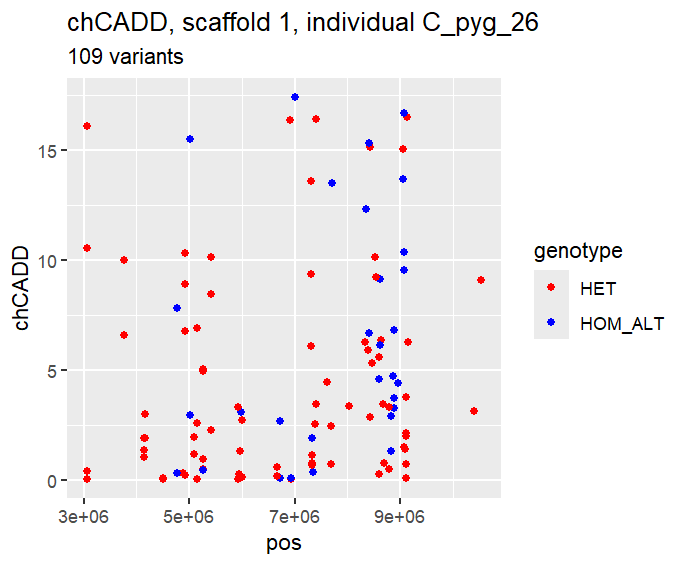
\includegraphics[width=0.8\textwidth]{img/chCADD_C_pyg_26.png}
    \caption{Rozkład wartości CADD wzdłuż scaffoldu 1 dla biegusa łyżkodziobego.}
    \label{fig:cadd_pyg}
\end{figure}

\begin{figure}[H]
    \centering
    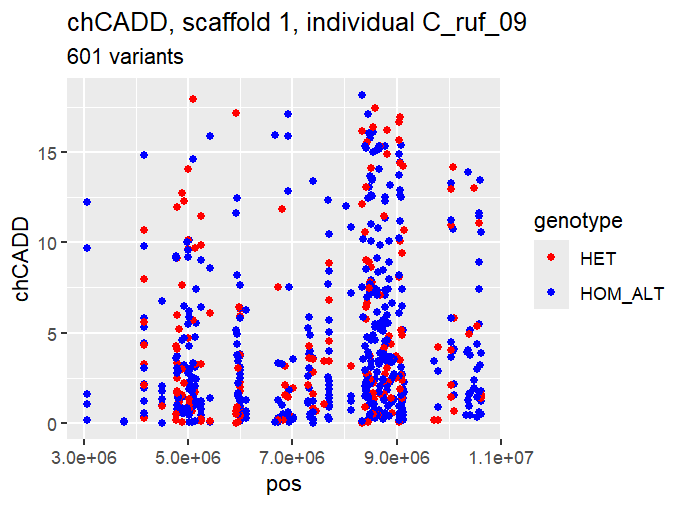
\includegraphics[width=0.8\textwidth]{img/chCADD_C_ruf_09.png}
    \caption{Rozkład wartości CADD wzdłuż scaffoldu 1 dla biegusa rdzawoszyjego.}
    \label{fig:cadd_ruf}
\end{figure}

\section{Dyskusja}
Wyniki wskazują, że biegus rdzawoszyi ma wyższe obciążenie genetyczne w porównaniu do biegusa łyżkodziobego, co może wynikać z większej liczby homozygotycznych wariantów. Jednak analiza ograniczyła się do jednego scaffoldu, co może nie odzwierciedlać sytuacji w całym genomie. Zastosowanie metod takich jak na zajęciach w hodowli w niewoli może zmniejszyć depresję wsobną i obciążenie genetyczne w populacjach zoo \cite{Speak2024}.

\bibliographystyle{plain}
\bibliography{references}

\end{document}